% !TEX encoding = UTF-8 Unicode
\RequirePackage{fix-cm}
\documentclass[a4paper,10pt,UTF8]{paper}
%\documentclass[a4paper,10pt,UTF8]{ctexart}

\usepackage[english]{babel}
\usepackage{fancyhdr,array,lastpage,amsmath,mathtools,enumitem,graphicx,multirow,tocbibind,longtable,makecell,varwidth,titlesec,bm,booktabs,comment,minted}
\usepackage{enumitem}
\usepackage{hyperref}
\hypersetup{hidelinks}




\usepackage[left=2.54cm,right=2.54cm,top=2.54cm,bottom=2.54cm]{geometry}
\usepackage[font=footnotesize,labelfont=bf]{caption}
\usepackage{tikz,flowchart}
\usepackage{ctex}
\usepackage{xeCJK}%中文字体
\usetikzlibrary{shapes,shapes.geometric,arrows,matrix,calc}
\usetikzlibrary{circuits.logic}

% \usetikzlibrary{circuits.logic.custom}
\usetikzlibrary{circuits.logic.IEC}
\usetikzlibrary{shadows}
\usepackage{listings}
\usepackage[Q=yes]{examplep}
\usepackage{fancyhdr}
\usepackage{alphalph}
\usepackage{indentfirst}

% \setCJKsansfont{黑体}
\setmainfont{PingFang SC}
\setCJKmainfont{PingFang SC}
\setCJKsansfont{PingFang SC}
\setmonofont{Monaco}

\newenvironment{sol}
  {\par\vspace{2mm}\noindent{\bf Solution}. }

\lstset{escapeinside=``, breaklines=true, frame=none, extendedchars=false, basicstyle=\ttfamily, showstringspaces=false}



\setlength{\parindent}{2em}
\setlength{\parskip}{1.5ex plus 0.5ex minus 0.2ex}
\linespread{1.1}

\bibliographystyle{plain}

\numberwithin{equation}{section}
\numberwithin{figure}{section}


\setcounter{secnumdepth}{3}
\setcounter{tocdepth}{3}

\title{华东师范大学计算机科学技术系上机实验报告}

\begin{document}
\pagestyle{fancy}
\chead{\small\color{gray}华东师范大学计算机科学技术系上机实验报告}
\lhead{}
\rhead{}
\makeatletter
\def\headrule{{\if@fancyplain\let\headrulewidth\plainheadrulewidth\fi%
\color{gray}\hrule\@height 0.2pt\@width\headwidth}
  \vspace{6mm}}
\makeatother

\definecolor{bg}{rgb}{0.95,0.95,0.95}
\newminted{asm}{bgcolor=bg}
\newminted{c}{bgcolor=bg}

\newcommand{\HRule}{\rule{\linewidth}{1mm}}
\newcommand{\dai}{\textbf{Dais-CMX16$^+$}}

{\center {\huge \bfseries \LARGE{华东师范大学计算机科学技术系上机实验报告}} \\ [0.8cm]

\small{
  \begin{minipage}[t]{.32\linewidth}
    \textbf{课程名称:}嵌入式系统\\
    \textbf{指导教师:}沈建华\\
    \textbf{上机实践名称:} 系统复位与时钟配置\\
    \textbf{实践编号:}实验5
  \end{minipage}
  \begin{minipage}[t]{.32\linewidth}
    \textbf{年级:}17 级\\
    \textbf{姓名:}朱桐\\
    \textbf{学号:}10175102111\\
  \end{minipage} 
  \begin{minipage}[t]{.32\linewidth}
    \textbf{上机实践成绩:} \\
    \textbf{创新实践成绩:} \\
    \textbf{上机实践日期:}2019/10/30\\
    \textbf{上机实践时间:}2 学时\\
  \end{minipage}
}
\HRule \\[0.5cm]
}


\section{实验目的}

\begin{enumerate}
    \item 进一步熟悉Keil实验环境,以及在连接开发板时Keil的相关配置
    \item 通过实验深入了解系统复位控制,包括外部复位、看门狗复位
    \item 通过实验掌握时钟配置
\end{enumerate}

\section{实验设备}

\begin{enumerate}
  \item 软件Keil5(keil提供了软件仿真功能);
  \item MSP432 P401R开发板
\end{enumerate}

\section{实验内容}

\begin{enumerate}
  \item 进一步熟悉Keil实验环境,以及在连接开发板时Keil的相关配置
  \item 通过实验深入了解系统复位控制,包括外部复位、看门狗复位
  \item 通过实验掌握时钟配置
\end{enumerate}


\section{实验原理}

\subsection{外部复位}

外部复位即RESET 引脚低电平,当复位引脚RESET作为开漏输入时,在复位引脚上宽度最小为500ns 的低电平脉冲即可产生一个外部复位。复位引脚RESET作为开漏输入时用于对外部设备进行复位。

\begin{figure}[h]
  \centering
  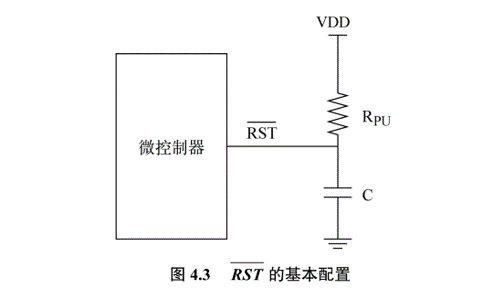
\includegraphics[width=0.6\textwidth]{1.png}
  \caption{}
  \label{}
\end{figure}

\subsection{看门狗复位}

看门狗定时器(Watch Dog Timer,WDT)与MCU 构成一个复位电路,这个电路一般有一个输入端和一个输出端,输入端用于“喂狗”,输出端接到MCU 的复位端。MCU正常工作的时候,每隔一端时间输出一个信号到“喂狗”端,使得看门狗计数器清零,如果超过规定的时间不喂狗,WDT 就会溢出并输出一个复位信号到MCU,使得MCU 复位,以防止MCU 死机。

\begin{figure}[h]
  \centering
  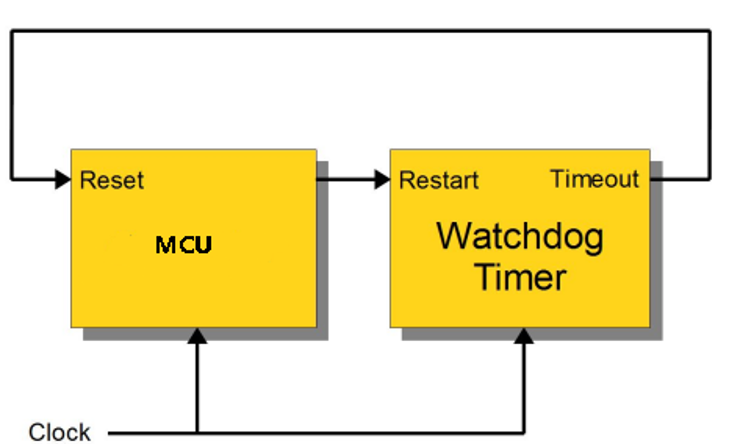
\includegraphics[width=0.6\textwidth]{2.png}
  \caption{看门狗复位}
  \label{}
\end{figure}


\subsection{MCLK 时钟配置}

MCLK为主时钟,用于CPU和片内外设。时钟系统模块的框图如下图 \ref{fig:3} 所示

\begin{figure}[h]
  \centering
  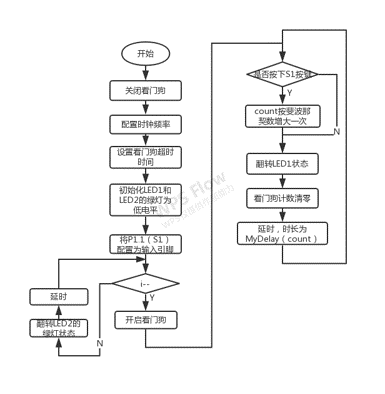
\includegraphics[width=0.6\textwidth]{3.png}
  \caption{时钟系统模块}
  \label{fig:3}
\end{figure}


主程序流程如图 \ref{fig:4}

\begin{figure}[h]
  \centering
  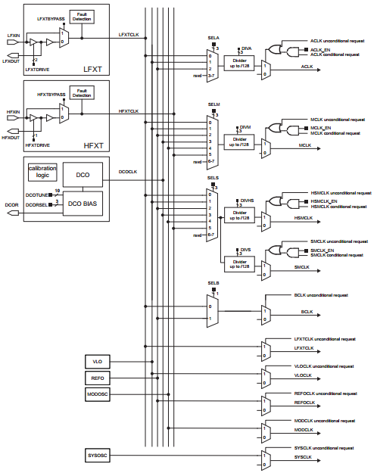
\includegraphics[width=0.3\textwidth]{4.png}
  \caption{主程序流程图}
  \label{fig:4}
\end{figure}


P1.1中断流程如图 \ref{fig:5}

\begin{figure}[h]
  \centering
  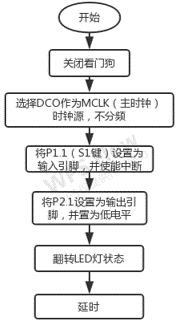
\includegraphics[width=0.3\textwidth]{5.png}
  \caption{P1.1中断流程图}
  \label{fig:5}
\end{figure}

\section{实验步骤}

\subsection{外部复位实验}

\begin{itemize}
  \item 使用keil 5新建工程,工程名的格式为: Lab0502\_Reset\_10175102111.uvprojx
  \item 控制LED1先长亮灭一次,再循环短亮灭。其中,第一次长亮灭要求灯亮时长定义为空循环600000次,即MyDelay(60),关于MyDelay函数的定义如下图;灯灭时长定义为空循环300000次。循环亮灭中,灯亮时长定义为空循环100000次,灯灭时长定义为空循环500000次。
  \item 按压开发板Reset(S3)按钮,观察实验现象
\end{itemize}


\subsection{看门狗复位实验}

\begin{itemize}
  \item 开发板的LED2(绿灯)先闪烁两次,然后LED1(红灯)周期性地闪烁;当按压键S1(P1.1)时,请按照斐波那契数列(1,1,2,3,5,8..)增大count值,count值用于延时函数MyDelay,即随着count值变化,LED1的闪烁周期变化;
  \item 不断按压键S1(P1.1),观察LED1(红灯)闪烁变化情况;
  \item 根据以上要求将工程05\_03补充完整,请思考此工程的功能实现有哪些可改进的地方。
\end{itemize}

\subsection{MCLK 时钟实验}

将工程05\_04编译烧写至开发板后,可以观察到LED2的绿灯以较快的频率闪烁;每次按 S1键后,会改变时钟分频,LED2的绿灯闪烁频率会逐步减慢;连续按压S1键8次后, LED2的绿灯又会以起始频率闪烁。

工程05\_04中使用DCO时钟源,LED2的绿灯闪烁频率是周期性地由快变慢,周期为8。请更换时钟源为MODCLK,LED2的绿灯闪烁频率改为周期性地由慢变快,周期为6,要求能明显观察到闪烁快慢变化。


\section{调试过程、结果与分析}

\subsection{外部复位实验}


新建工程时,我们需要导入一些外部代码如图 \ref{fig:6}, \ref{fig:7}

\begin{figure}[h]
  \centering
  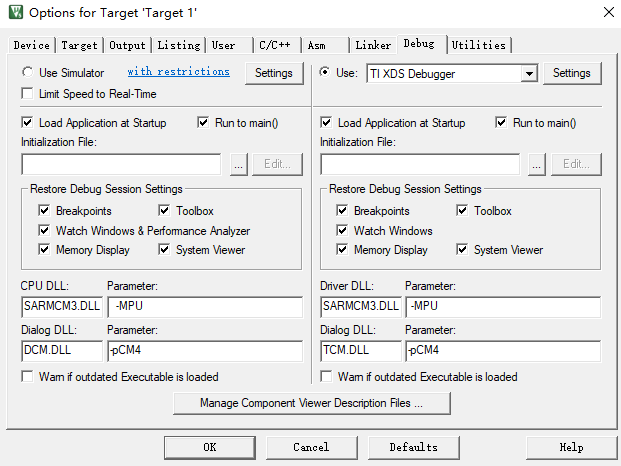
\includegraphics[width=0.6\textwidth]{6.png}
  \caption{调试器配置}
  \label{fig:6}
\end{figure}

\begin{figure}[h]
  \centering
  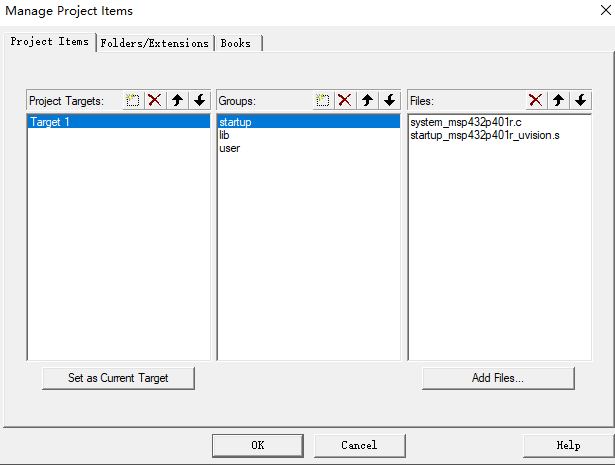
\includegraphics[width=0.3\textwidth]{7.png}
  \caption{项目信息配置}
  \label{fig:7}
\end{figure}



\begin{ccode}
  GPIO_toggleOutputOnPin(GPIO_PORT_P1,GPIO_PIN0);
    MyDelay(60);
    GPIO_toggleOutputOnPin(GPIO_PORT_P1,GPIO_PIN0);
    MyDelay(30);

  while (1) {
    GPIO_toggleOutputOnPin(GPIO_PORT_P1,GPIO_PIN0);
    MyDelay(10);
    GPIO_toggleOutputOnPin(GPIO_PORT_P1,GPIO_PIN0);
    MyDelay(50);
  }
\end{ccode}

其中 GPIO\_toggleOutputOnPin(GPIO\_PORT\_P1,GPIO\_PIN0); 可以改变 LED1 的暗灭状态,我们就用这个函数控制亮灭

\subsection{看门狗复位实验}

定义我们需要的变量

\begin{ccode}
  //*-----------在此下区域可定义变量-----------*//
    unsigned i=4;
    unsigned int count=1, fn, fn1 = 1, fn2 = 0;
  //*-----------在此上区域可定义变量-----------*//  
\end{ccode}

计算斐波那契数列

\begin{ccode}
  //*-----------在此下区域修改-----------*//
  //检测到P1.1按键被按下
  if (GPIO_getInputPinValue(GPIO_PORT_P1, GPIO_PIN1)==GPIO_INPUT_PIN_LOW)
  {
      count = fn = fn1 + fn2;
      fn2 = fn1;
      fn1 = fn;
  }
  //*-----------在此上区域修改-----------*//
\end{ccode}

实际上不会因为斐波那契数列的无限增长而停止闪烁,因为会存在看门狗复位。程序中设置超过两秒会清零

\begin{ccode}
  //设置看门狗超时时间为2s,即2s内看门狗计数器未清理零则复位LaunchPad,
  // t=WDT/SMCLK=32K/16K=2
    MAP_WDT_A_initWatchdogTimer(WDT_A_CLOCKSOURCE_SMCLK,
    WDT_A_CLOCKDIVIDER_32K);
\end{ccode}

当周期太长的时候,程序控制流会停在 MyDelay 函数而不会到达下面的 MAP\_WDT\_A\_clearTimer() 函数,从而引发看门狗复位

\begin{ccode}
  while(1)
  {
    //*-----------在此下区域修改-----------*//
    //检测到P1.1按键被按下
    if (GPIO_getInputPinValue(GPIO_PORT_P1, GPIO_PIN1)==GPIO_INPUT_PIN_LOW)
    {
      count = fn = fn1 + fn2;
      fn2 = fn1;
      fn1 = fn;
    }
    //*-----------在此上区域修改-----------*//
    
    GPIO_toggleOutputOnPin(GPIO_PORT_P1,GPIO_PIN0); //翻转P1.0电平,
    // 翻转红色LED1电平
    MAP_WDT_A_clearTimer(); //看门狗计数清零
    MyDelay(count);
  }
\end{ccode}


\subsubsection{改进}

实验要求并没有给定改进的目标,为了检查效果改进代码并未添加在工程文件。这里假定希望能实现更长周期的斐波那契数列,那么我们需要停用看门狗计数器

\begin{ccode}
  /* 停用看门狗定时器 */
  MAP_WDT_A_holdTimer();
\end{ccode}

使用更高的数据类型记录斐波那契数列

\begin{ccode}
  
  //延时函数
  void MyDelay(unsigned long long count)
  {
    volatile unsigned long long i;
    for(i=1000*count; i>0; i--);
    return ;
  }
  ////.....
  unsigned long long fn, fn1=1, fn2=0;
\end{ccode}

\subsection{MCLK 时钟实验}

改变时钟源

\begin{ccode}
  /* 配置时钟频率MCLK=3M(主时钟频率) DCO默认频率3M*/   
  MAP_CS_initClockSignal(CS_MCLK, CS_MODOSC_SELECT, CS_CLOCK_DIVIDER_128); 
\end{ccode}

改变周期为6

\begin{ccode}
  count++;
  count%=6;
\end{ccode}

改编为由快到慢需要两个地方,一个是初始速度,一个是每个 count 数值对应的速度

\begin{ccode}
  /* 配置时钟频率MCLK=3M(主时钟频率) DCO默认频率3M*/   
  MAP_CS_initClockSignal(CS_MCLK, CS_MODOSC_SELECT, CS_CLOCK_DIVIDER_128); 
  //////...
  switch(count)
  {
    case 0:
      tmp=CS_CLOCK_DIVIDER_128; //不分频
      break;
    case 1:
      tmp=CS_CLOCK_DIVIDER_64; //2分频,以下类推
      break;
    case 2:
      tmp=CS_CLOCK_DIVIDER_32;
      break;
    case 3:
      tmp=CS_CLOCK_DIVIDER_16;
      break;
    case 4:
      tmp=CS_CLOCK_DIVIDER_8;
      break;
    case 5:
      tmp=CS_CLOCK_DIVIDER_4;
      break;           
    default:
      return ;
  }
\end{ccode}

\section{总结}

http://www.ti.com/ 有很多额外的参考资料,对 msp432p401r 开发大有帮助

\section{附件}

\end{document}
